\section{Introduction}
One of the major goals of the global neutrino physics programme is to explore why we live in a matter-dominated universe. Charge-parity symmetry violation (CPV) in the neutrino sector is one of the few remaining possibilities to be explored experimentally. 
CPV searches compare the probabilities of $\nu_{\mu}\!\rightarrow\!\nu_e$ and $\overline{\nu}_{\mu}\!\rightarrow\!\overline{\nu}_e$ oscillation, which, in the absence of CPV, should be equal. 
To convert the measured rate of interactions to a level of CPV, experiments must accurately know the cross section for the interactions of neutrinos and anti-neutrinos with detector materials, most importantly hydrogen, carbon, oxygen, iron and argon. 
Therefore, systematic uncertainties on neutrino-nucleus interaction cross sections are a key input to such CPV searches.  
These interaction cross-sections are dependent on theoretical models because the target nucleon resides in a complicated nucleus, and the nuclear model has dramatic effects on the measured final-state particle kinematic distributions. JOCELYN:"Citation needed"

The strongest current constraint on CPV in neutrinos, from the T2K experiment, reports neutrino interaction systematic uncertainties at the 5--8\% level \cite{Abe:2018wpn}.
The future DUNE and Hyper-K projects assume systematic errors at the 1--2\% level to achieve their physics goals, but will be in the same position as current experiments ($>$5\% errors) if the nuclear-model uncertainties are not reduced.  
The key to reducing these uncertainties is to precisely measure the multiplicity and momentum distribution of final-state particles. 
However these distributions are modified by final state interactions (FSI) of the recoiling secondary particles as they leave the target nucleus.  
The most commonly used neutrino generator Monte Carlos (GENIE~\cite{Andreopoulos:2009rq}, NEUT~\cite{Hayato:2009zz}, and NuWro~\cite{GOLAN2012499}), simulate FSI with cascade models that are tuned with external hadron-nucleus scattering measurements.
\begin{figure}%
    \centering
    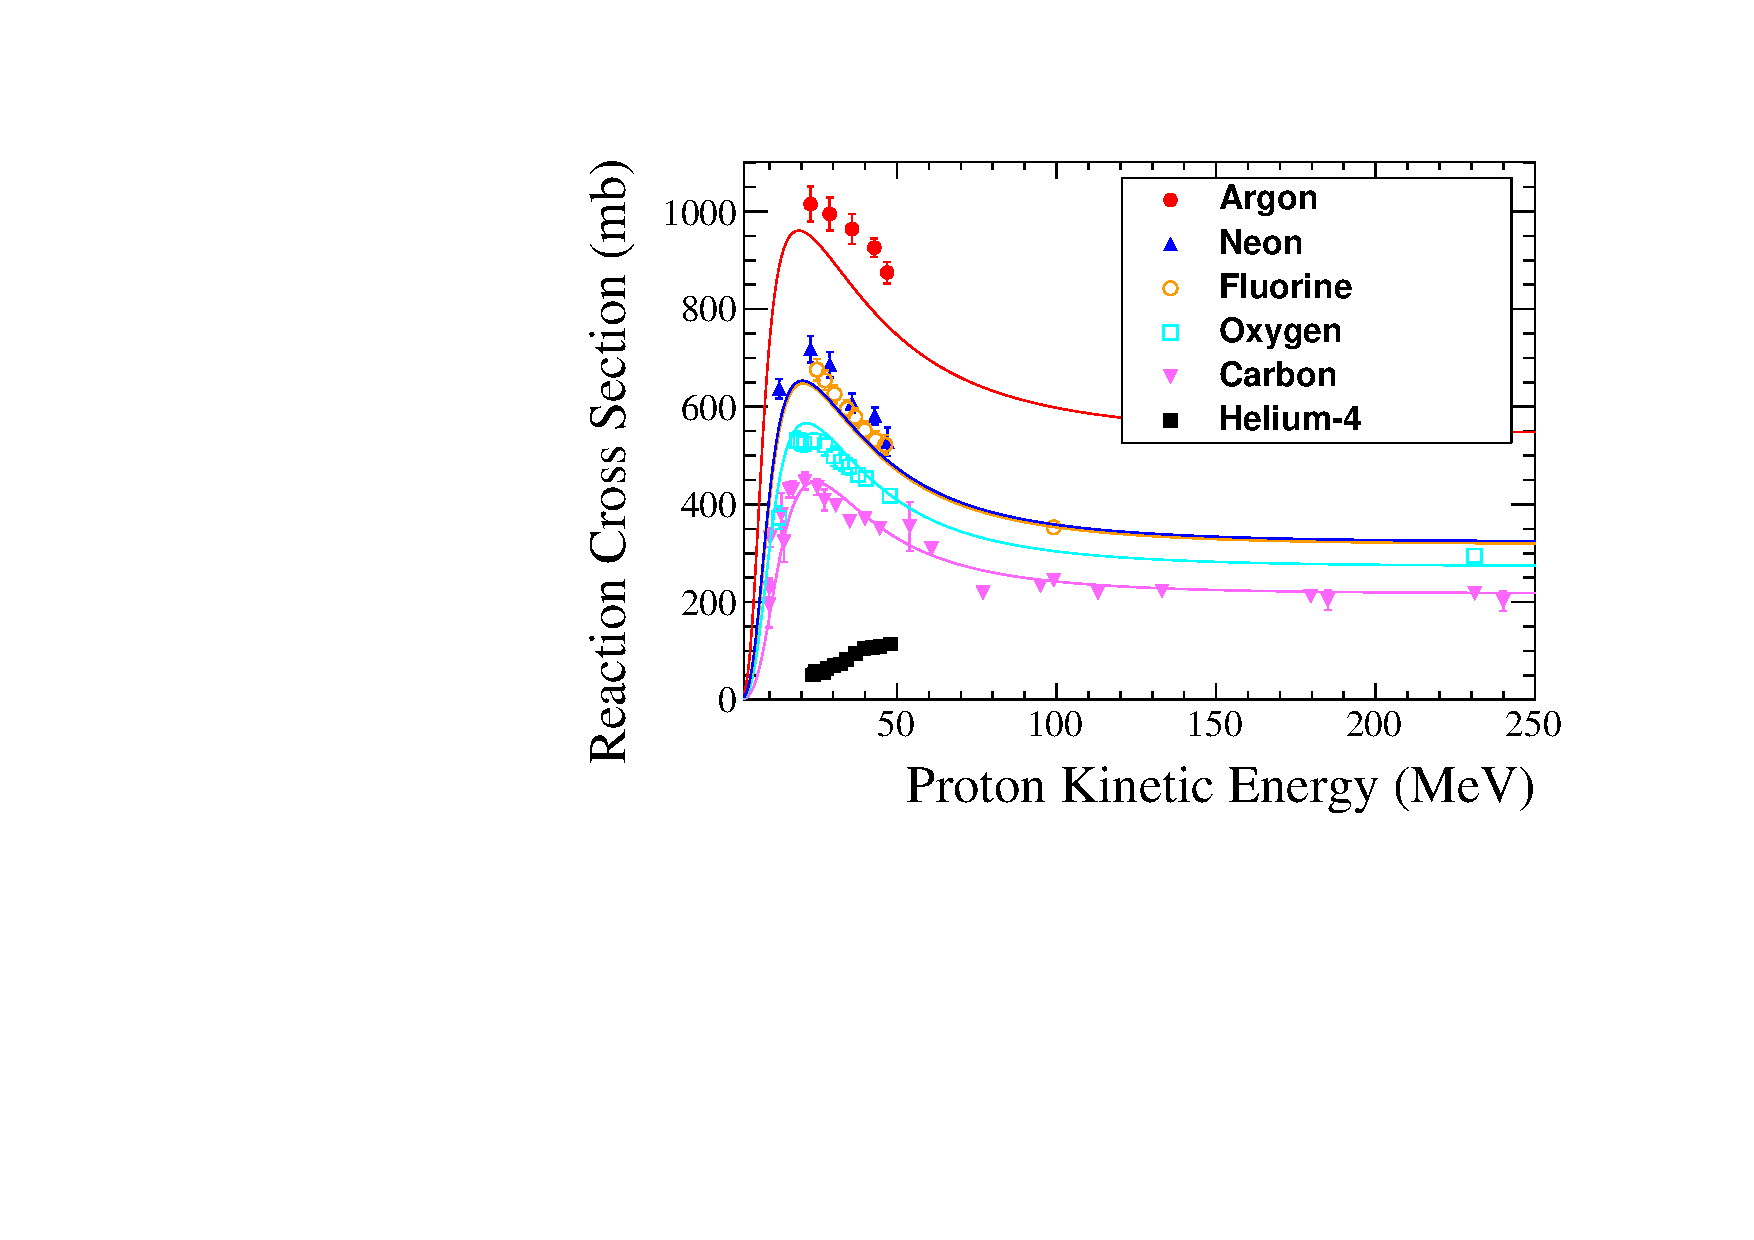
\includegraphics[width=12cm]{files/Figures/DataProtonCrossSections.pdf}%
    \caption{Total reaction cross-sections for protons on  argon, neon, fluorine, oxygen, carbon, and helium-4. JOCELYN:"Citation needed for data as well as model" Data is shown against a semi-empirical model from Wellisch and Axen~\cite{wellisch1996total}.}
    \label{fig:DataProtonXSec}%
\end{figure}

However, as shown in Figure~\ref{fig:DataProtonXSec}, these proton-nucleus scattering measurements are extremely sparse and in many cases do not exist in the relevant momentum region and/or on the relevant nuclei.
Therefore semi-empirical parameterisations are used to extrapolate in momentum and atomic mass.  
The parametrisations are different between the three generators, and yield order-of-magnitude scale differences in the predicted multiplicity and kinematics of final state protons.
The proton final state modeling is a key ingredient for neutrino oscillation measurements because it affects the event selection and neutrino energy reconstruction in charged-current interactions, which is the channel used to measure oscillation parameters and therefore central to the search for CP violation JOCELYN:"Citation needed".  
For these reasons, FSI contribute dominantly to the total neutrino interaction systematic uncertainty~\cite{Abe:2018wpn}.

Further, FSI models are in tension with data.  
Recent neutrino scattering measurements have shown that the most-used models of neutrino-nucleus interactions (employed by NEUT and GENIE) differ from nature in both cross section and kinematics of final state particles by as much as 30\%~\cite{Wascko:2009cn,Wascko:2011hy}. 
These errors cannot be fully mitigated with near/far detector combinations because they come from theoretical model deficiencies that are not cancelled in the ratio~\cite{Coloma:2013rqa}. 
To achieve 1-2\% systematics for CPV searches, interaction models must be tuned and validated against precise proton-nucleus and pion-nucleus scattering measurements covering a broad final-state particle phase space, on a range of nuclear targets~\cite{Cao:2014zra}.

\begin{figure}%
    \centering
    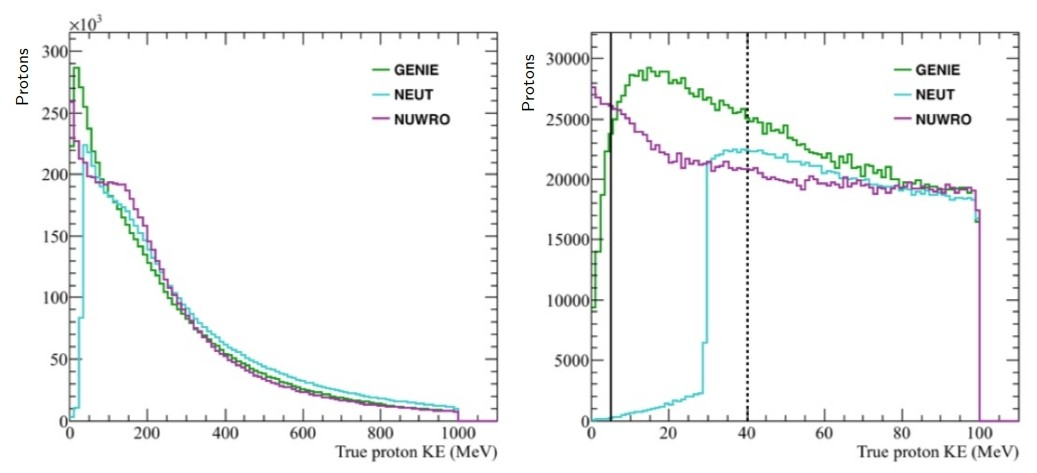
\includegraphics[width=12cm]{files/Figures/protons_from_argon.jpeg}%
    \caption{JOCELYN:"which target, what energy, more details" Predicted proton energy spectra from GENIE, NEUT, and NUWRO. Energy spectra up to 1 GeV are shown on the left, and zoomed in to lower energies on the right. The dashed vertical line indicates the expected proton automated-reconstruction/ID threshold in liquid argon, and the solid vertical line shows the same for gaseous argon at 10 atm. The lower threshold in high pressure gas provides a unique opportunity to distinguish among the models for the same nuclear target.}
    \label{fig:protonsfromargon}%
\end{figure}
% TPCs are ideal for such measurements because of the 4$\pi$ angular coverage of all final state particles with high efficiency and low momentum thresholds, which are the keys to distinguish between models.  
The key proton kinetic energy range in which to distinguish between interaction models is the region below 50 GeV.
Figure~\ref{fig:protonsfromargon} shows the proton multiplicity and kinetic energy distributions for $\nu_{\mu}$ charged-current (CC) interactions on argon calculated by the GENIE, NEUT, and NuWro neutrino generators JOCELYN"What neutrino flux is assumed?".  
These distributions are highly discrepant, particularly in the fraction of events with few ejected protons, and at low proton kinetic energy, below 50 MeV.
This is predominately below the proton detection threshold in liquid Argon TPCs (40 MeV) and in water Cherenkov detectors (500 MeV).
%The threshold for a well-reconstructed proton in argon gas at 5 (10) bar is 3 MeV (5 MeV), and therefore such a detector could accurately probe the key low-momentum region of parameter space to reduce neutrino interaction cross section uncertainties. 
%This measurement range is highly complementary to what can be learned from liquid argon detectors. 

We have built a High Pressure gas Time Projection Chamber (HPTPC) prototype and exposed it to a charged particle beam at the T10 beamline in CERN in August and September 2018 \cite{SPSC-P-355}.
JOCELYN:"before this next statement i think you need a figure (or a sentence) that shows (describes) the typical T10 beam spectrum (before we did anything with it), and explains that the low-momentum flux is negligble."
The physics objective of the beam test was to make measurements of low momentum protons in argon, at lower momenta than were available in the T10 beamline. 

To enhance the low energy proton flux, a novel technique was used:
we placed acrylic moderator blocks directly in the beamline, which spread the beam particles, via multiple Coulomb scattering. JOCELYN:"Throughout the introduction, stick to proton KE or momentum (probably KE because of plots)"
By placing the TPC in an off-axis position, we achieved a beam composition with lower-momentum protons than would otherwise have been possible in the T10 beamline.
These techniques were designed to increase the ratio of protons to the beam's minimum ionizing particle (MIP) background in the TPC, while also decreasing the proton momentum and multiplicity in the active region of the TPC.

The flux and composition of beam particles produced via scattering in the acrylic moderator blocks was measured with two time of flight (ToF) systems, placed upstream and downstream of the TPC.
Measurements of protons and minimum ionizing particles are presented as a function of the off axis angle, distance from the moderator, and thickness of the moderator.
%This paper provides a detailed description of the time of flight systems, followed by an analysis of the ToF data yielding particle flux predictions.
This paper provides a detailed description of the time of flight systems and beamline in Section 2,  the analysis methodology of the ToF data in section 3, presentation of the ToF system results in Section 4, and additional conclusions in Section 5.